% Created 2021-08-13 Fri 16:02
% Intended LaTeX compiler: pdflatex
\documentclass[11pt]{article}
\usepackage[utf8]{inputenc}
\usepackage[T1]{fontenc}
\usepackage{graphicx}
\usepackage{grffile}
\usepackage{longtable}
\usepackage{wrapfig}
\usepackage{rotating}
\usepackage[normalem]{ulem}
\usepackage{amsmath}
\usepackage{textcomp}
\usepackage{amssymb}
\usepackage{capt-of}
\usepackage{hyperref}
\author{Sreejith Sreekumar}
\date{\today}
\title{Linear Model}
\hypersetup{
 pdfauthor={Sreejith Sreekumar},
 pdftitle={Linear Model},
 pdfkeywords={},
 pdfsubject={},
 pdfcreator={Emacs 26.3 (Org mode 9.1.9)}, 
 pdflang={English}}
\begin{document}

\maketitle
\tableofcontents

\begin{itemize}
\item Sklearn's \('train\_test\_split'\) should not be used as data is time series
\item Pythons' indexing is used instead
\item In stats models, a constant has to be added manually to include the bias term
\item In linear regression p-values are obtained as a result of a t-test on the co-efficients
\item p-value is the percent chance that a coefficient is actually zero. i,e it has no effect on the target
\end{itemize}


\section{Splitting the data}
\label{sec:orgb8b479d}

\begin{verbatim}

# Import the statsmodels.api library with the alias sm
import statsmodels.api as sm

# Add a constant to the features
linear_features = sm.add_constant(features)

# Create a size for the training set that is 85% of the total number of samples
train_size = int(0.85 * features.shape[0])
train_features = linear_features[:train_size]
train_targets = targets[:train_size]
test_features = linear_features[train_size:]
test_targets = targets[train_size:]
print(linear_features.shape, train_features.shape, test_features.shape)

\end{verbatim}


\section{Building the model}
\label{sec:orgf6cf335}

\begin{verbatim}
# Create the linear model and complete the least squares fit
model = sm.OLS(train_targets, train_features)
results = model.fit()  # fit the model
print(results.summary())

# examine pvalues
# Features with p <= 0.05 are typically considered significantly different from 0
print(results.pvalues)

# Make predictions from our model for train and test sets
train_predictions = results.predict(train_features)
test_predictions = results.predict(test_features)
\end{verbatim}

\begin{center}
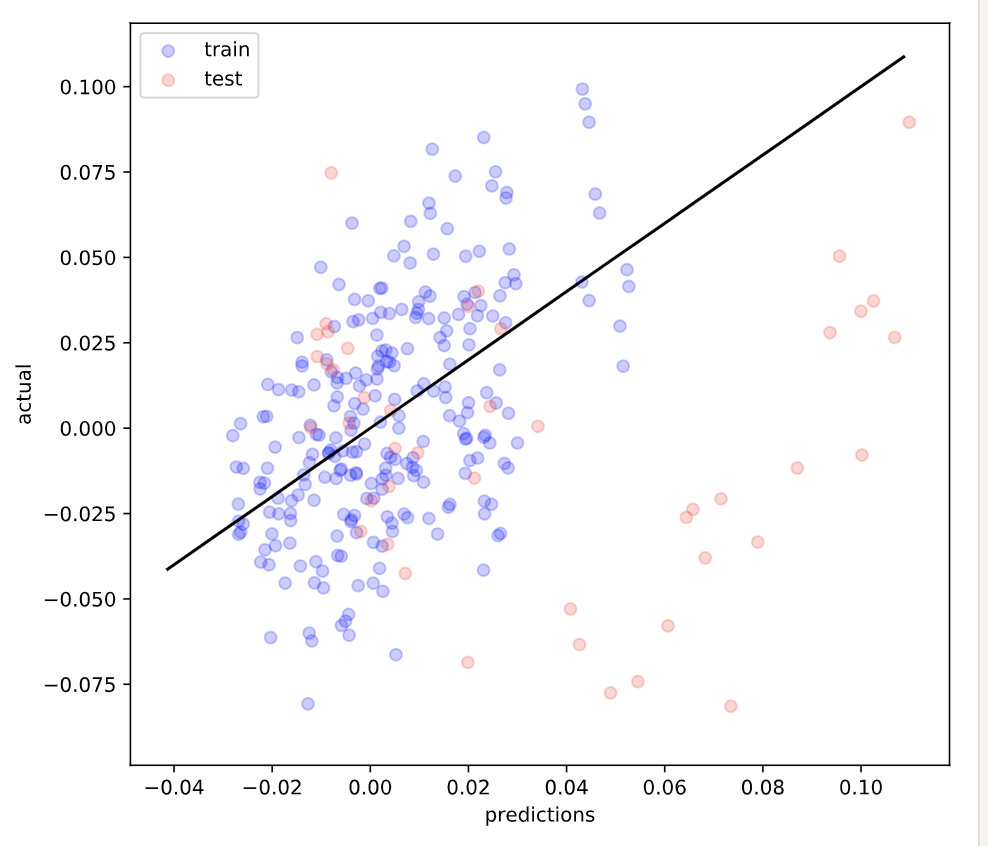
\includegraphics[width=.9\linewidth]{linear-model.png}
\end{center}
\end{document}